\chapter{Projeto Conceitual do Produto}

\section{Características gerais}

\textcolor{black}{O projeto foi dividido em 4 frentes (\textit{Estrutura}, \textit{Hardware}, \textit{Software} e \textit{Consumo Energético}), com o intuito de organizar e estruturar o mesmo de forma que os objetivos sejam alcançados de maneira eficiente e segura, seguindo os requisitos estabelecidos previamente pela equipe e pelos orientadores.
As atribuições das 3 frentes serão realizadas conjuntamente, de modo a garantir que a integração e o funcionamento das mesmas esteja de acordo com o esperado inicialmente pela equipe.}

\textcolor{black}{A frente de \textbf{\textit{Estrutura}} será responsável pela definição, aquisição e montagem dos materiais necessários para elaboração da estrutura do carrinho. Para alcançar os objetivos previstos, a estrutura apresentada deverá sustentar e proteger um ovo de galinha durante a execução dos trajetos determinados, e, logicamente, ser desenvolvida de forma com que o carrinho consiga completar os mesmos. }

\textcolor{black}{A frente de \textbf{\textit{Hardware}} será responsável pela definição, aquisição e configuração dos componentes eletrônicos que serão utilizados na elaboração do carrinho, além de garantir a medição de dados em tempo real para trajetória percorrida, velocidade instantânea, aceleração instantânea, tempo de percurso e consumo energético.}

\textcolor{black}{A frente de \textbf{\textit{Software}} será responsável pela definição, documentação e programação dos códigos que serão utilizados para definir o funcionamento do carrinho, além de realizar os cálculos e armazenamento dos dados de trajetória percorrida, velocidade instantânea, aceleração instantânea, tempo de percurso e consumo energético.}



\textcolor{black}{A frente de \textbf{\textit{Consumo Energético}}  será responsável pela definição, aquisição e montagem dos componentes que alimentarão o carrinho e seus demais componentes, além de efetuar o cálculo e medições dos relacionados ao consumo energético do mesmo.}

\begin{figure}[htpb]
\centering
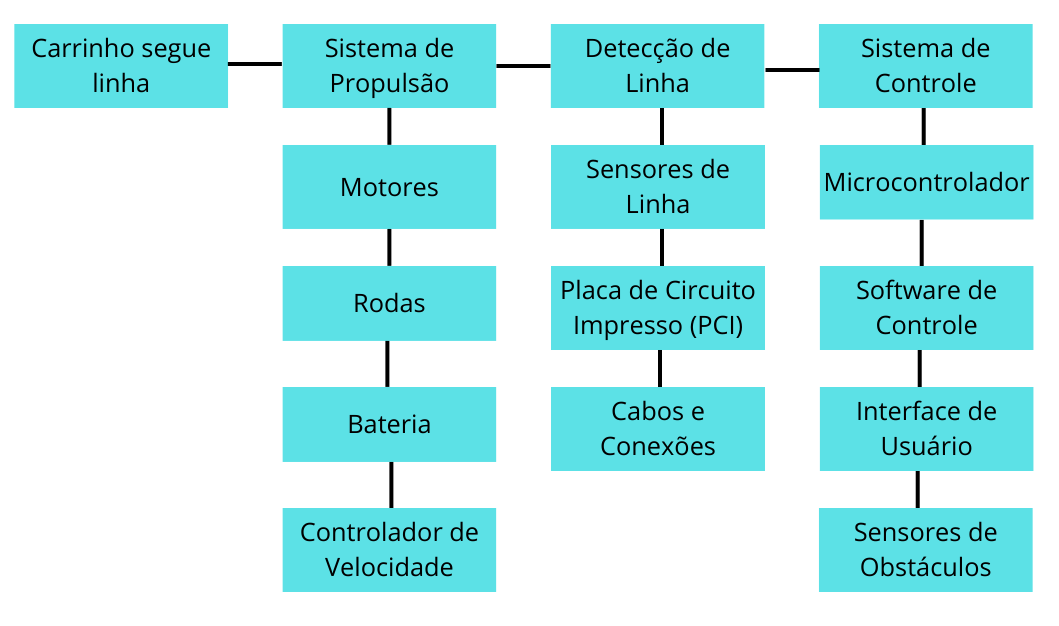
\includegraphics[width=\textwidth]{figuras/EAP.png}
\caption{Estrutura Analítica do Projeto.}
\label{EAP}
\end{figure}

%\textcolor{red}{Apresentar e explicar a Estrutura Analítica do Projeto (EAP), tomando cuidado com a legibilidade da imagem. Se necessário, coloque a EAP dentro do comando ``\textsf{\textbackslash begin\{landscape\} \textbackslash end\{landscape\}}'' para que ela seja apresentada em uma página deitada.}

\subsection{Itens teóricos}

\textcolor{black}{Para o desenvolvimento do projeto, diversos fatores devem ser levados em consideração de forma a facilitar a integração entre as frentes e a orientação do projeto como um todo. A \textbf{coleta e a análise dos dados coletados} deverão ser feitas de maneira precisa e coerente, utilizando técnicas e ferramentas que permitam persistir e agrupar os valores obtidos em variáveis de banco de dados, de forma a atender requisitos previamente estabelecidos para distância e tempo.}

\textcolor{black}{ As atividades realizadas pelas frentes serão integradas e, por isto, deverão ser executadas com rigor e exigem uma comunicação constante e eficaz entre as partes, visando garantir uma melhor desenvolvimento do produto. As frentes de \textbf{Software e Hardware} deverão trabalhar juntas no que diz respeito a integração dos circuitos e componentes eletrônicos com os códigos e programas responsáveis pelos movimentos e cálculos necessários para o projeto.}

\textcolor{black}{A frente de \textbf{Consumo Energético}, trabalhará em conjunto com ambas, visando entender quais os componentes e configurações necessárias para que o funcionamento do carrinho esteja otimizado e o mais adequado possível.}

\textcolor{black}{A frente de \textbf{Estrura}, trabalhará em contato com a frente de \textbf{\textit{Hardware e Consumo Energético}}, visando compreender as necessidades estruturais para que o carrinho comporte os componentes eletrônicos e energéticos necessários para seu funcionamento e para que os requisitos previamente estabelecidos sejam atendidos.}

\section{Estrutura}

\textcolor{red}{Apresentar desenho em CAD, indicar dimensões por lado/aresta/cota, indicar materiais utilizados e explicar o desenho e as decisões de projeto.}

\section{Descrição de \textit{hardware}}

\textcolor{red}{A descrição de hardware no documento deve permitir que outras pessoas repliquem o produto proposto neste documento. Para isso, indiquem:}

\textcolor{red}{\begin{itemize}
    \item O diagrama de blocos \cite{blockdiagram}, que oferece uma visão geral do hardware, com as principais partes do sistema e as ligações entre elas.
    \item A lista de materiais \cite{bom}, que facilita a montagem do sistema, indicando tudo que deve ser adquirido. Aproveitem a lista de materiais para apresentarem o orçamento dos mesmos.
    \item O esquemático \cite{esquematico}, que mostra as conexões elétricas entre os componentes. Deve-se indicar os componentes por nomes e símbolos, e as conexões entre eles, incluindo a pinagem dos componentes. Se o esquemático ficar muito grande, pode-se separa-lo em vários esquemáticos. A ligação em \textit{protoboard} não é considerada um esquemático adequado.
\end{itemize}}

\textcolor{red}{Além de mostrar tudo isso, é necessário organizar a descrição de \textit{hardware} no texto, e explicar as escolhas feitas. Comece com o diagrama de blocos, que é mais genérico, e depois indiquem os detalhes com a lista de materiais e os esquemáticos.}

\section{Análise de consumo energético}

\textcolor{red}{Com relação ao consumo energético do produto desenvolvido, será necessário apresentar cálculos de consumo dos diversos componentes utilizados e explicar as decisões de projeto para atender a estas demandas.}

\section{Descrição de \textit{software}}

\textcolor{red}{Com relação ao \textit{software}, será necessário apresentar os seguintes itens: % pacotes de componentes de \textit{software}, suas funções e características, e explicar as decisões de projeto:
\begin{enumerate}
    \item Um diagrama do processo de negócio do problema que a máquina se propõe a resolver (BPNM) – não é UML, mas é fundamental para entender como o sistema se comporta como um todo, incluindo o usuário;
    \item Lista de casos de uso (backlog do sistema). Backlog funcional;
    \item Lista de requisitos não-funcionais a serem satisfeitos pelo sistema;
    \item Diagrama de casos de uso: mostrando os requisitos funcionais, seus atores e como eles interagem entre si;
    \item Diagrama de Classes: apresentando quais dados são manipulados pelo sistema (internamente e externamente – ex.: resultados de experimentos);
    \item Diagrama de arquitetura, identificando todos os componentes da máquina e suas iterações com o software;
    \item Diagrama de estados da máquina (sistema);
    \item Descrição dos testes dos componentes da máquina e dos testes funcionais que deveriam ser feitos para avaliar o funcionamento da máquina e identificar defeitos. São importantes os testes unitários (componentes) e de integração (conjunto de componentes) e o roteiro de testes.
\end{enumerate}
}
%\textcolor{red}{Com relação ao \textit{software}, será necessário apresentar pacotes de componentes de \textit{software}, suas funções e características, e explicar as decisões de projeto.}

